\documentclass[a4paper,12pt]{article}
\usepackage[utf8x]{inputenc}
\usepackage[romanian]{babel}
%\usepackage[T2A]{fontenc}
\usepackage{amsmath}
\usepackage{amsfonts}
\usepackage{amssymb}
\usepackage[hidelinks]{hyperref}
\usepackage{tikz}
	\usetikzlibrary{matrix,positioning}
%===============================================================================
\usepackage{ntheorem}
  \theoremstyle{change}
  \theorembodyfont{\upshape}
  \newtheorem{theorem}{Teoremă}[section]
  \newtheorem{definition}[theorem]{Definiție}
  \newtheorem{example}[theorem]{Exemplu}
  \newtheorem{proposition}[theorem]{Propoziție}
  \newtheorem{corollary}[theorem]{Corolar}
  \newtheorem{remark}[theorem]{Remarcă}
%  \newenvironment{proof}{{\bf Demonstrație:} }{}
  %\newtheorem{exercise}[theorem]{Exercițiu}
\newenvironment{proof}[1][Proof]{\begin{trivlist}
\item[\hskip \labelsep {\bfseries #1}]}{\end{trivlist}}  
  \newtheorem{question}[theorem]{\^{I}ntrebare}
  \newtheorem{problem}[theorem]{Problemă}
  \newtheorem{algorithm}[theorem]{Algoritm}
%===============================================================================
\usepackage{verbatim}
\usepackage{graphicx}
\usepackage{hyperref}
\usepackage{color}
\usepackage{caption}
\usepackage{subcaption}
%===============================================================================
\usepackage{titlesec}
  \titleformat{\chapter}
    {\normalfont\huge\bfseries}{}{20pt}{\Huge}
  \titlespacing*{\chapter}{0pt}{50pt}{40pt}
  \titleclass{\section}{straight}
\usepackage{xargs}
\usepackage{minibox}% http://tex.stackexchange.com/questions/8680/how-can-i-insert-a-newline-in-a-framebox
  \renewcommandx\minibox[3][1=l, 2=c]{%
    \begin{tabular}[#2]{@{}#1@{}}
      #3
    \end{tabular}%
  }
%===============================================================================

%===============================================================================
\usepackage{exercise}
  \renewcommand{\ExerciseName}{}
  \renewcommand{\ExerciseListName}{}
  \renewcommand{\ExerciseHeaderTitle}{\ExerciseTitle}
  \renewcommand{\ExerciseHeader}{\textbf{
                \ExerciseName\ExerciseHeaderNB.\ExerciseHeaderTitle
                \ExerciseHeaderOrigin}}
  \renewcommand{\ExerciseHeader}{\textbf{
                \ExerciseName\ExerciseHeaderNB.\ExerciseHeaderTitle}}
  \renewcommand{\ExerciseListHeader}{\ExerciseHeaderDifficulty%
              \textbf{\ExerciseListName\ \ExerciseHeaderNB.%
              \ \ExerciseHeaderTitle}%
              \ExerciseHeaderOrigin\ignorespaces}
  \renewcommand{\ExerciseListHeader}{\ExerciseHeaderDifficulty%
              \textbf{\ExerciseListName\ \ExerciseHeaderNB.%
              \ \ExerciseHeaderTitle}%
              \ignorespaces}
  \setlength{\ExerciseSkipBefore}{0\baselineskip}
  \setlength{\ExerciseSkipAfter}{0\baselineskip}
  \setlength{\Exesep}{0\baselineskip}
  \setlength{\Exetopsep}{0\baselineskip}
  \setlength{\Exeleftmargin}{25em}
  \setlength{\QuestionBefore}{0\baselineskip}
%===============================================================================

\newcommand{\N}[1]{\mathbb{#1}}




\title{Elemente de analiză funcțională\\Note de curs}
\author{Radu N. Dumbraveanu}

\begin{document}

\maketitle

\tableofcontents

%===============================================================================
\section{Săptămâna 7}
%===============================================================================

%-------------------------------------------------------------------------------
\subsection{Obiectul analizei funcționale}
%-------------------------------------------------------------------------------

% Spaţii metrice. Exemple. Inegalităţile Young, Holder, Minkowski.

%-------------------------------------------------------------------------------
\subsection{Spații metrice}
%-------------------------------------------------------------------------------

%-------------------------------------------------------------------------------
\subsection{Inegalităţile Young, H\"older, Minkowski}
%-------------------------------------------------------------------------------

% Mulţimi închise şi mulţimi deschise. Spaţii metrice separabile.

%-------------------------------------------------------------------------------
\subsection{Mulțimi deschise}
%-------------------------------------------------------------------------------

%-------------------------------------------------------------------------------
\subsection{Mulțimi închise}
%-------------------------------------------------------------------------------

%-------------------------------------------------------------------------------
\subsection{Spații metrice separabile}
%-------------------------------------------------------------------------------

%===============================================================================
\section{Săptămâna 8}
%===============================================================================

% Convergenţa într-un spaţiu metric. Şiruri fundamentale.

%-------------------------------------------------------------------------------
\subsection{Convergență}
%-------------------------------------------------------------------------------

%-------------------------------------------------------------------------------
\subsection{Șiruri Cauchy (sau fundamentale)}
%-------------------------------------------------------------------------------

% Spaţii metrice complete. Exemple.

%-------------------------------------------------------------------------------
\subsection{Spații complete}
%-------------------------------------------------------------------------------

\begin{theorem}
Fie $A$ o submulțime a unui spațiu metric $(X,d)$. Atunci:
\begin{enumerate}
\item $x\in cl A$ dacă și numai dacă există un șir $(x_n)$ din $A$ astfel încît $lim x_n = x$;
\item $A$ este închisă dacă și numai dacă „$(x_n)\subseteq A$, $lim x_n = x$” implică $x\in A$.
\end{enumerate}
\end{theorem}

\begin{proof}
Fie $x\in cl A$. Dacă $x\in A$ atunci $x,x,x,...$ este șirul căutat. Dacă $x\notin A$ atunci pentru orice $n=1,2,...$ bila $B(x,\frac{1}{n})$ conține un $x_n\in A$. Rezultă că $\lim x_n = x$ deoarece $\frac{1}{n}\to 0$ atunci cînd $n\to\infty$.

Dacă $x_n\in A$ și $x_n\to x$ atunci $x\in A$ sau orice vecinătate a lui $x$ conține puncte $x_n\neq x$, adică $x$ este un punct de acumulare a lui $A$. Așadar $x\in cl A$.

Mulțimea $A$ este închisă dacă $A=cl A$. Rezultă din cele de mai sus.
\end{proof}

\begin{theorem}\label{thm:subspatiu-complet}
Fie $X$ un spațiu metric complet și $A$ un subspațiu al lui $X$. Atunci $A$ este complet dacă și numai dacă $A$ este închis în $X$.
\end{theorem}

\begin{proof}
Fie $A$ complet atunci pentru orice $x\in cl A$ există $(x_n)\subseteq A$ astfel încît $\lim x_n=x$. Dar atunci întrucîț $(x_n)$ este Cauchy, iar $A$ este complet rezultă că $(x_n)$ converge în $A$. Din unicitatea limitei rezultă $x\in A$, adică $A=cl A$.

Fie $A$ închisă și $(x_n)$ un șir Cauchy. Atunci, întrucît $X$ este complet, $\lim x_n = x\in X$. Deoarece $A$ este închisă rezultă că $x\in cl A = A$. Așadar orice șir Cauchy din $A$ converge în $A$. Deci $A$ este complet.
\end{proof}

%-------------------------------------------------------------------------------
\subsection{Spații complete remarcabile}
%-------------------------------------------------------------------------------

\paragraph{Spațiile $\mathbb{R}^n$ și $\mathbb{C}^n$} Spațiul euclidian $\mathbb{R}^n$ și spațiul unitar $\mathbb{C}^n$ sunt complete.

\begin{proof}[Într-adevăr]
Vom considera mai întâi spațiul $\mathbb{R}^n$.
Și reamintim că metrica pe $\mathbb{R}^n$ (metrica euclidiană) este definită prin 

\[ d(x,y) = \left(\sum_{i=1}^n (\xi_i - \eta_i)^2\right)^\frac{1}{2} \]

\noindent unde $x=(\xi_i)$ și $y=(\eta_i)$. 

Fie $(x_m)$ un șir Cauchy în $\mathbb{R}^n$, cu $x_m=(\xi_1^{(m)},\xi_2^{(m)},...,\xi_n^{(m)})$. Atunci pentru orice $\varepsilon$ pozitiv, există un rang $m_{\varepsilon}$ astfel încît pentru toți termenii $x_m$ și $x_p$ de rang mai mare decît $m_{\varepsilon}$ ($m,p>m_{\varepsilon}$) să avem

\begin{equation}\label{l1}
d(x_m,x_p) = \left(\sum_{i=1}^n (\xi_i^{(m)}-\eta_i^{(p)})^2\right)^\frac{1}{2} < \varepsilon.
\end{equation}

Ridicînd la pătrat ambele părți ale inegalității obținem

\[ \sum_{i=1}^n (\xi_i^{(m)}-\eta_i^{(p)})^2 < \varepsilon^2. \]

Întrucît termenii sumei sînt nenegativi reiese că pentru orice $m,p>m_\varepsilon$ și $i=\overline{1,n}$ avem

\[ (\xi_i^{(m)}-\eta_i^{(p)})^2 < \varepsilon^2 \text{ și respectiv } |\xi_i^{(m)}-\eta_i^{(p)}| < \varepsilon. \]

Din ultima relație rezultă că pentru fiecare $i=\overline{1,n}$,  șirul de numere reale $\xi_i^{(1)}, \xi_i^{(2)}, ..., \xi_i^{(m)}, ...$ este un șir Cauchy. Acest șir este convergent, conform criteriului Cauchy de convergență a șirurilor numerice: $\xi_i^{(m)}\to \xi_i$ cînd $m\to\infty$. Folosind aceste $n$ limite definim $x=(\xi_1,\xi_2,...,\xi_n)$. Evident, $x\in\mathbb{R}^n$. Trecînd la limită în \eqref{l1} cu $p\to\infty$ pentru $m>m_\varepsilon$ avem

\[ d(x_m,x)\leq\varepsilon. \]

Așadar $x$ este limita șirului $(x_m)$ și întrucît acest șir a fost ales arbitrar spațiul $\mathbb{R}^n$ este complet.

Completitudinea spațiului $\mathbb{C}^n$ se demonstrează analog.

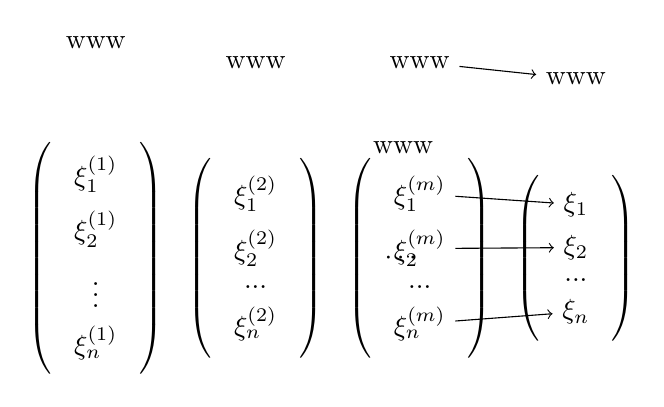
\begin{tikzpicture}
	[
		every matrix/.style={matrix of math nodes, left delimiter = ( ,right delimiter = )}
	]
	\matrix(mx1) at (0,0)
	{
		\xi_1^{(1)} \\
		\xi_2^{(1)} \\
		\vdots\\
		\xi_n^{(1)} \\
	};
	\matrix(mx2) [right = of mx1]
	{
		\xi_1^{(2)} \\
		\xi_2^{(2)} \\
		...\\
		\xi_n^{(2)} \\
	};
	\node(mxdots) [right = of mx2] {$\cdots$};
	\matrix(mxm) [right = of mx2]
	{
		\xi_1^{(m)} \\
		\xi_2^{(m)} \\
		...\\
		\xi_n^{(m)} \\
	};
	\matrix(mx) [right = of mxm]
	{
		\xi_1 \\
		\xi_2 \\
		...\\
		\xi_n \\
	};

%	\node(x1) [above = of mx1] {$x_1$};
%	\node(x2) [above = of mx2] {$x_2$};
%	\node(xdots) [above = of mxdots] {$\cdots$};
%	\node(xm) [above = of mxm] {$x_m$};
%	\node(x) [above = of mx] {$x$};	
	\foreach \x in {1,2,dots,m,{}}
		\node(x\x) [above = of mx\x]{www};
	
	\draw[->] (xm) -- (x);
	\foreach \x in {1,2,4} {\draw[->] (mxm-\x-1) -- (mx-\x-1);};
\end{tikzpicture}

\end{proof}

\paragraph{Spațiul $l^\infty$} Spațiul $l^\infty$ este complet.

\begin{proof}[Într-adevăr]

Fie $(x_m)$ un șir Cauchy în $l^\infty$, unde $x_m=(\xi_1^{(m)},\xi_2^{(m)},...)$. Întrucît metrica pe $l^\infty$ este definită prin

\[ d(x,y) = \sup_{i=1}^{\infty} |\xi_i - \eta_i| \]

\noindent unde $x=(\xi_i)$ și $y=(\eta_i)$, iar $(x_m)$ este Cauchy, pentru orice $\varepsilon$ pozitiv, există un rang $n_{\varepsilon}$ astfel încît pentru toți termenii $x_m$ și $x_n$ de rang mai mare decît $m_{\varepsilon}$ ($m,n>m_{\varepsilon}$) să avem

\[ d(x_m,x_n) = \sup_{i=1}^{\infty} |\xi_i^{(m)} - \xi_i^{(n)}| < \varepsilon. \]

Deoarece supremul este luat de la elemente nenegative reiese că pentru orice $m,n>m_\varepsilon$ și $i$ fixat avem

\[
\label{l2}
|\xi_i^{(m)} - \xi_i^{(n)}| < \varepsilon.
\]

Din ultima relație reies că pentru fiecare $i$ șirul de numere reale (complexe) $\xi_i^{(1)}, \xi_i^{(2)}, ..., \xi_i^{(m)}, ...$ este un șir Cauchy. Acest șir converge conform criteriului Cauchy de convergență a șirurilor numerice: $\xi_i^{(m)}\to \xi_i$ cînd $m\to\infty$. Folosind aceste limite infinite definim $x=(\xi_1,\xi_2,...)$. Vom arăta că $x\in l^\infty$ și $x_m\to x$.

Trecînd la limită în \eqref{l2} cu $n\to\infty$ avem

\[
\label{l2star}
|\xi_i^{(m)} - \xi_i| \leq \varepsilon.
\]

Întrucîț $x_m=(\xi_i^{(m)})\in l^\infty$ reiese că $(x_m)$ este mărginit, i.e. există un număr real $k_m$ încît pentru orice $i$ avem $|\xi_i^{(m)}|\leq k_m$. Astfel aplicînd inegalitatea triunghiului obținem ($m>m_\varepsilon$)

\[
|\xi_i|=|\xi_i-\xi_i^{(m)}+\xi_i^{(m)}|\leq |\xi_i-\xi_i^{(m)}|+|\xi_i^{(m)}|\leq\varepsilon+k_m
\]

Inegalitatea de mai sus este adevărată pentru orice $i$ și din cauza că în membrul drept $i$ nu este prezent rezultă că șirul $(\xi_i)$ este mărginit, i.e. $x\in l^\infty$. De asemenea din \eqref{l2star} pentru $m>m_\varepsilon$ obținem

\[
d(x_m,x)=\sup_i |\xi_i^{(m)}-\xi_i|\leq \varepsilon.
\]

Rezulta că $x_m\to x$. Așadar $l^\infty$ este complet.

\end{proof}

\paragraph{Spațiul $c$} Spațiul $c$ este complet. 

\begin{proof}
Reamintim că $c$ este spațiul șirurilor convergente de numere reale sau complexe.
Metrica acestuia este cea indusă din $l^\infty$ deoarece $c$ este subspațiu al lui $l^\infty$.
Vom utiliza Teorema~\ref{thm:subspatiu-complet}, adică vom arăta că $c$ este un subspațiu închis în $l^\infty$.

Fie $x=(\xi_i)\in cl(c)$. Atunci există $x_m=(\xi_i^{(m)})\in c$ astfel încît $x_m\to x$ cînd $m\to\infty$. Adică pentru orice $\varepsilon$ pozitiv, există un rang $m_{\varepsilon}$ astfel încît pentru toți termenii $x_m$ de rang mai mare decît $m_{\varepsilon}$ ($m>m_{\varepsilon}$) să avem

\[
  d(x_m,x) = \sup_{i=1} |\xi_i^{(m)} - \xi_i| < \varepsilon
\]

Deoarece supremul este luat de la elemente nenegative reiese că pentru orice $m>m_\varepsilon$ și $i$ fixat avem

\[
|\xi_i^{(m)} - \xi_i| < \frac{\varepsilon}{3}.
\]

Pe de altă parte, $\xi_i^{(m)}$ sînt coordonate ale punctelor din $c$, adică de șiruri (de numere reale sau complexe) convergente. Rezultă că fiecare șir $\xi_1^{(m)}, \xi_2^{(m)}, ...$ este Cauchy. Deci pentru orice $\varepsilon$ pozitiv, există un rang $i_{\varepsilon}$ astfel încît pentru toți termenii $\xi_i^{(m)}$ și $\xi_j^{(m)}$ de rang mai mare decît $i_{\varepsilon_1}$ ($i,j>i_{\varepsilon}$) să avem

\[
|\xi_i^{(m)}-\xi_j^{(m)}|<\frac{\varepsilon}{3}
\]

Aplicăm inegalitatea triunghiului pentru orice $i,j>i_\varepsilon$:

\[
|\xi_i-\xi_j|<|\xi_i^{(m)}|+|\xi_i^{(m)}-\xi_j^{(m)}|+|\xi_j^{(m)}-\xi_j|<\varepsilon.
\]

Rezultă că $(\xi_i)$ este șir convergent, i.e. $x=(x_i)\in c$. Așadar $x\in cl(c)$.
\end{proof}

\paragraph{Spațiul $l^p$} Spatiul $l^p$ este complet, $1\leq p<\infty$.

\begin{proof}
Fie $(x_m)$ un șir Cauchy în $l^p$, unde $x_m=(\xi_1^{(m)},\xi_2^{(m)},...)$. Întrucît metrica pe $l^p$ este definită prin

\[
  d(x,y) = \left(\sum{i=1}^\infty |\xi_i - \eta_i|^p\right)^{\frac{1}{p}}
\]

\noindent unde $x=(\xi_i)$ și $y=(\eta_i)$, iar $(x_m)$ este Cauchy, pentru orice $\varepsilon$ pozitiv, există un rang $m_{\varepsilon}$ astfel încît pentru toți termenii $x_m$ și $x_n$ de rang mai mare decît $m_{\varepsilon}$ ($m,n>m_{\varepsilon}$) să avem

\[
\label{l3}
d(x_m,x_n) = \left(\sum_{i=1}^\infty |\xi_i^{(m)} - \xi_i^{(n)}|^p\right)^{\frac{1}{p}} < \varepsilon.
\]

Deoarece suma este luată de la elemente nenegative reiese că pentru orice $m,n>m_\varepsilon$ și $i$ fixat avem

\[
\label{l4}
|\xi_i^{(m)} - \xi_i^{(n)}| < \varepsilon.
\]

Dacă în \eqref{l4} fixăm $i$ reiese că șirul $\xi_i^{(1)},\xi_i^{(2)},...$ este Cauchy. Și respectiv este convergent deoarece $\mathbb{R}$ și $\mathbb{C}$ sînt spații complete. Fie $\xi_i^{(m)}\to \xi_i$ cînd $m\to\infty$. Folosind aceste limite definim $x=(\xi_1, \xi_2,...)$. Vom arăta că $x\in l^p$ și că $x_m\to x$.

Din \eqref{l3} (ridicînd la puterea $p$) avem pentru orice $m,n>m_\varepsilon$:

\[
\sum_{i=1}^r |\xi_i^{(m)} - \xi_i^{(n)}|^p < \varepsilon^p.
\]

Trecînd la limită cu $n\to\infty$ pentru $m>m_\varepsilon$ avem

\[
\sum_{i=1}^r |\xi_i^{(m)} - \xi_i|^p \leq \varepsilon^p.
\]

Acum trecînd la limită cu $r\to\infty$:

\[
\label{l5}
\sum_{i=1}^\infty |\xi_i^{(m)} - \xi_i|^p \leq \varepsilon^p.
\]

Ultima inegalitate arată că: $x_m-x=(\xi_i^{(m)}-\xi_i)\in l^p$. Întrucîț $x_m\in l^p$ din inegalitatea lui Minkowski reiese:

\[
x=x_m+(x-x_m)\in l^p.
\]

Mai mult, seria din \eqref{l5} reprezintă $[d(x_m,x)]^p$ și deci \eqref{l5} implică $x_m\to x$.

\end{proof}

\paragraph{Spațiul $C[a,b]$} Spațiul de funcții continue $C[a,b]$ este complet; $[a,b]$ interval închis în $\mathbb{R}$.

\begin{proof}
Fie $(x_m)$ un șir Cauchy în $C[a,b]$, unde $x_m=x_m(t)$, $t\in [a,b]$. Întrucîț metrica pe $C[a,b]$ este definită prin

\[
  d(x,y) = max_{t\in [a,b]} |x(t)-y(t)|
\]

\noindent unde $x=x(t)$ și $y=y(t)$ și $(x_m)$ este Cauchy, pentru orice $\varepsilon$ pozitiv, există un rang $m_{\varepsilon}$ astfel încît pentru toți termenii $x_m$ și $x_n$ de rang mai mare decît $m_{\varepsilon}$ ($m,n>m_{\varepsilon}$) să avem:

\[
\label{l6}
d(x_m,x_n) = max_{t\in [a,b]} |x_m(t)-x_n(t)|<\varepsilon
\]

Atunci pentru orice $t_0\in [a,b]$:

\[
|x_m(t_0)-x_n(t_0)|<\varepsilon.
\]

Reiese că $x_1(t_0),x_2(t_0),...$ este un șir numeric Cauchy. Întrucît $\mathbb{R}$ este complet acest șir converge. Fie $x_m(t_0)\to x(t_0)$ cînd $m\to\infty$. În așa fel pentru orice $t\in[a,b]$ putem asocia un număr $x(t)$. Astfel am definit punctual o funcție $x$ pe $[a,b]$. Vom arata că $x\in C[a,b]$ și $x_m\to x$.

Trecînd la limită în \eqref{l6} cu $n\to\infty$ obținem

\[
max_{t\in [a,b]} |x_m(t)-x(t)|\leq \varepsilon
\]

Deci pentru orice $t$

\[
|x_m(t)-x(t)|\leq \varepsilon
\]

Ultima inegalitate arată că $(x_m(t))$ converge uniform către $x(t)$ pe $[a,b]$. Deoarece $x_m(t)$ sînt continue și convergența este uniformă rezultă că și limita $x(t)$ este continuă.
\end{proof}


% Completarea spaţiilor metrice. Teorema Hausdorff.

%-------------------------------------------------------------------------------
\subsection{Completarea spațiilor metrice}
%-------------------------------------------------------------------------------

\begin{definition}
Două spații metrice $(X,d)$ și $(\tilde{X}, \tilde{d})$ se numesc \emph{izomorfe} dacă există o aplicație bijectivă $h:X\longrightarrow \hat{X}$, numită \emph{izomorfism}, astfel încît pentru orice $x$ și $y$ din $X$ să avem 
\[
	d(x,y)=\tilde{d}(h(x),h(y)).
\]
\end{definition}

\begin{theorem}
Pentru orice spațiu metric $(X, d)$ există un spațiu metric complet $(\hat{X}, \hat{d})$ și o izometrie $h$ între $X$ și $\hat{X}$ astfel încît $h(X)$ este un subspațiu dens în $\hat{X}$. 

Spațiul $(\hat{X},\hat{d})$ este unic pînă la o izometrie de spații metrice, adică dacă $\tilde{X}$ este un spațiu metric complet cu un subspațiu dens $\tilde{W}$ isometric cu $X$ atunci $\tilde{X}$ și $\hat{X}$ sînt izometrice.
\end{theorem}

\begin{proof}
Vom prezenta numai o schiță de demonstrație.

Pentru orice două șiruri Cauchy $(x_n)$ și $(x_n')$ din $X$ definim relația de echivalență $\sim$: $(x_n)\sim(x_n')$ dacă și numai dacă $lim_{n\to\infty}d(x_n,x_n')=0$.

Fie $\hat{X}$ mulțimea claselor de echivalență $\hat{x}$, $\hat{y}$ în raport cu acestă relație. Fie 
\[
	\hat{d}(\hat{x},\hat{y})=\lim_{n\to\infty}(x_n,y_n)
\]
unde $(x_n)\in\hat{x}$ și $(y_n)\in\hat{y}$.

Construim izometria $h$ astfel pentru orice $x\in X$ îi asociem $\hat{x}$ astfel încît șirul constant $(x,x,x,x,...)\in \hat{x}$
\end{proof}

\begin{remark}
Spațiul $(\hat{X},\hat{d})$ construit în teorema precedentă se numește \emph{completatul} spațiului $(X,d)$.
\end{remark}

%-------------------------------------------------------------------------------
\subsection{Teorema Hausdorff}
%-------------------------------------------------------------------------------

% Teorema lui Cantor. Mulţimi rare. Teorema Baire.

%-------------------------------------------------------------------------------
\subsection{Teorema lui Cantor}
%-------------------------------------------------------------------------------

%-------------------------------------------------------------------------------
\subsection{Mulțimi rare}
%-------------------------------------------------------------------------------

%-------------------------------------------------------------------------------
\subsection{Teorema Baire}
%-------------------------------------------------------------------------------

% Aplicaţii de contracţie. Principiul punctului fix. Aplicații generalizate de  contracţie. Aplicaţii generalizate de  contracţie. Aplicaţii ale principiului  punctului fix.

%-------------------------------------------------------------------------------
\subsection{Contracții}
%-------------------------------------------------------------------------------

%-------------------------------------------------------------------------------
\subsection{Principiul punctului fix}
%-------------------------------------------------------------------------------

%-------------------------------------------------------------------------------
\subsection{Aplicaţii ale principiului  punctului fix}
%-------------------------------------------------------------------------------

%===============================================================================
\section{Săptămâna 9}
%===============================================================================

% Mulţimi compacte. Teorema Hausdorf  şi consecinţele ei.

%-------------------------------------------------------------------------------
\subsection{Compactitate}
%-------------------------------------------------------------------------------

\url{http://www.ucl.ac.uk/~ucahad0/3103_handout_2.pdf}

%-------------------------------------------------------------------------------
\subsection{Teorema Hausdorf}
%-------------------------------------------------------------------------------

% Criterii de cmpacitate în C  a,b  Acoperiri. Teorema Borel. Funcţii continui    pe mulţimi compacte.

%-------------------------------------------------------------------------------
\subsection{Criterii de cmpacitate în $C[a,b]$}
%-------------------------------------------------------------------------------

\url{http://www.math.psu.edu/wysocki/M403/Notes403_10.pdf}

\begin{definition}
Familia de funcții continue $\mathcal{F}\subseteq C[a,b]$ se numește \emph{echicontinuă} dacă pentru orice $f\in \mathcal{F}$ și  $\varepsilon$ pozitiv există $\delta$ pozitiv astfel încît
\[
|f(x)-f(y)|<\varepsilon\text{ pentru orice }x,y\in[a,b]\text{ cu }d(x,y)<\delta. 
\]
\end{definition}
Fie $X$ un spațiu metric compact. O submulțime $\mathcal{F}\subseteq C(X)$ este relativ compactă dacă și numai dacă $\mathcal{F}$ este echicontinuă și echimărginită.
\begin{theorem}

\end{theorem}

%-------------------------------------------------------------------------------
\subsection{Teorema Borel}
%-------------------------------------------------------------------------------

%-------------------------------------------------------------------------------
\subsection{Funcții continui pe mulțimi compacte}
%-------------------------------------------------------------------------------

% Spaţii liniare normate. Subspaţii. Sume directe şi subspaţii.

%-------------------------------------------------------------------------------
\subsection{Norma}
%-------------------------------------------------------------------------------

% Spaţii Banah. Spaţii cât.

%-------------------------------------------------------------------------------
\subsection{Spații Banach}
%-------------------------------------------------------------------------------

%-------------------------------------------------------------------------------
\subsection{Spații cît}
%-------------------------------------------------------------------------------

%===============================================================================
\section{Săptămâna 10}
%===============================================================================

% Izomorfizmul spaţiilor normate finit dimensionale. Spaţiile L    şi L

%-------------------------------------------------------------------------------
\subsection{Izomorfizmul spaţiilor normate finit dimensionale}
%-------------------------------------------------------------------------------

%-------------------------------------------------------------------------------
\subsection{Spaţiile $L$ și $L$}
%-------------------------------------------------------------------------------

% Spaţii  Hilbert. Spaţii prehilbertiene.

%-------------------------------------------------------------------------------
\subsection{Spaţii  Hilbert}
%-------------------------------------------------------------------------------

%-------------------------------------------------------------------------------
\subsection{Spaţii prehilbertiene}
%-------------------------------------------------------------------------------

% Operatori liniari şi mărginiţi. Exemple.

%-------------------------------------------------------------------------------
\subsection{Operatori liniari}
%-------------------------------------------------------------------------------

%-------------------------------------------------------------------------------
\subsection{Operatori mărginiţi}
%-------------------------------------------------------------------------------

% Norma operatorului  liniar. Exemple.

%-------------------------------------------------------------------------------
\subsection{Norma operatorului liniar}
%-------------------------------------------------------------------------------

%===============================================================================
\section{Săptămâna 11}
%===============================================================================

% Spaţiul operatoriloi liniari. Principiul mărginirii uniforme.

%-------------------------------------------------------------------------------
\subsection{Spațiul operatorilor liniari}
%-------------------------------------------------------------------------------

%-------------------------------------------------------------------------------
\subsection{Principiul mărginirii uniforme}
%-------------------------------------------------------------------------------

% Convergenţa tare a şirului de operatori. Prelungirea operatorilor liniari.

%-------------------------------------------------------------------------------
\subsection{Convergenţa tare a şirului de operatori}
%-------------------------------------------------------------------------------

%-------------------------------------------------------------------------------
\subsection{Prelungirea operatorilor liniari}
%-------------------------------------------------------------------------------

% Funcţionale liniare. Exemple.

%-------------------------------------------------------------------------------
\subsection{Funcționale liniare}
%-------------------------------------------------------------------------------

% Prelungirea funcţionalelor liniare. Teorema Hahn-Banach.

%-------------------------------------------------------------------------------
\subsection{Prelungirea funcționalelor liniare}
%-------------------------------------------------------------------------------

%-------------------------------------------------------------------------------
\subsection{Teorema Hahn-Banach}
%-------------------------------------------------------------------------------

%===============================================================================
\section{Săptămâna 12}
%===============================================================================

% Forma generală a funcţionalelor liniare şi mărginite în unele spaţii finitdimensionale.

%-------------------------------------------------------------------------------
\subsection{Forma generală a funcţionalelor liniare}
%-------------------------------------------------------------------------------

% Forma generală a funcţionalelor în spaţiile Ca,b şi  Lp  a,b

%-------------------------------------------------------------------------------
\subsection{Forma generală a funcţionalelor în spaţiile }
%-------------------------------------------------------------------------------

% Convergenţa slabă. Teorema Polya-Steclov.

%-------------------------------------------------------------------------------
\subsection{Convergenţa slabă}
%-------------------------------------------------------------------------------

%-------------------------------------------------------------------------------
\subsection{Teorema Polya-Steclov}
%-------------------------------------------------------------------------------

% Măsura mărimilor elementare. Măsura Lebesgue a mulţimilor plane.

%-------------------------------------------------------------------------------
\subsection{Măsura mărimilor elementare}
%-------------------------------------------------------------------------------

%-------------------------------------------------------------------------------
\subsection{Măsura Lebesgue a mulțimilor plane}
%-------------------------------------------------------------------------------

%===============================================================================
\section{Săptămâna 13}
%===============================================================================

% Noţiuni generale despre măsură. Prelungirea măsurii de pe un inel. - aditivitatea măsurii. Prelungirea Lebesque  a măsurii.

%-------------------------------------------------------------------------------
\subsection{Măsura}
%-------------------------------------------------------------------------------

%-------------------------------------------------------------------------------
\subsection{Prelungirea Lebesque a măsurii}
%-------------------------------------------------------------------------------

% Funcţiile măsurabile. Teorema Egorov şi teorema Luzin. 

%-------------------------------------------------------------------------------
\subsection{Funcțiile măsurabile}
%-------------------------------------------------------------------------------

%-------------------------------------------------------------------------------
\subsection{Teorema Egorov şi teorema Luzin}
%-------------------------------------------------------------------------------

% Funcţii simple . Integrala Lebesque

%-------------------------------------------------------------------------------
\subsection{Funcții simple}
%-------------------------------------------------------------------------------

%-------------------------------------------------------------------------------
\subsection{Integrala Lebesgue}
%-------------------------------------------------------------------------------

% -aditivitate şi trecerea la limită sub semnul integralei Lebesque.

%-------------------------------------------------------------------------------
\subsection{Trecerea la limită sub semnul integralei Lebesgue}
%-------------------------------------------------------------------------------

%===============================================================================
\section{Săptămâna 14}
%===============================================================================

% Legătura între integrala Lebesque şi integrala Riemann. Funcţii cu variaţie mărginită.

%-------------------------------------------------------------------------------
\subsection{Legătura între integrala Lebesgue şi integrala Riemann}
%-------------------------------------------------------------------------------

% Produsul sistemului de mulţimi, produsul măsurilor.

%-------------------------------------------------------------------------------
\subsection{Produsul măsurilor}
%-------------------------------------------------------------------------------

% Măsura Stiltes. Integrala Lebesque-Stiltes. Integrala Riemann-Stiltes.

%-------------------------------------------------------------------------------
\subsection{Măsura Stiltjes}
%-------------------------------------------------------------------------------

% Trecerea la limită sub semnul integralei Stiltes.

%-------------------------------------------------------------------------------
\subsection{Trecerea la limită sub semnul integralei Stiltjes}
%-------------------------------------------------------------------------------

%===============================================================================
\section{Săptămâna 15}
%===============================================================================

\end{document}